\documentclass{standalone}
\usepackage{tikz,pgfplots,calc}
\usetikzlibrary{positioning,calc}
\usetikzlibrary{arrows}
\usepackage{tkz-euclide}
\usetkzobj{all}


\begin{document}
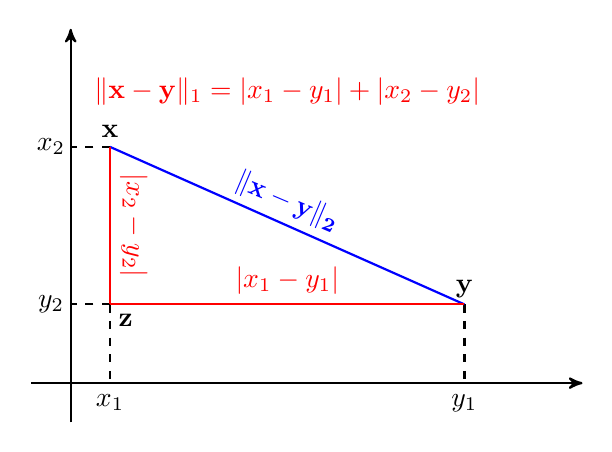
\begin{tikzpicture}[>=stealth', thick]


    % \node (p0) at (-2, 0) {};
    % \node [anchor

    \def\xx{.5}
    \def\xy{3}
    \def\yx{5}
    \def\yy{1}
    \coordinate (p0) at (0, 0) {};
    \coordinate (x) at (\xx, \xy);
    \coordinate (y) at (\yx, \yy);

    \coordinate (xy) at (\xx, \yy);
    \draw [->] (-.5, 0) --++ (7, 0);
    \draw [->] (0, -.5) --++ (0, 5);


    \draw [dashed] (xy) --(\xx, 0);
    \draw [dashed] (x) --++(-\xx, 0);
    \node at (\xx, \xy + .2) {$\mathbf{x}$};
    \node at (\yx, \yy + .2) {$\mathbf{y}$};
    \node at (\xx + .2, \yy - .2) {$\mathbf{z}$};
    \node at (\xx, -.25) {$x_1$};
    \node at (\yx, -.25) {$y_1$};
    \node at (-.25, \xy) {$x_2$};
    \node at (-.25, \yy) {$y_2$};
    \node [rotate = -23] at (.5*\xx + .5*\yx, .5*\xy + .5*\yy + .3) {\textcolor{blue}{$\mathbf{\|\mathbf{x - y}\|_2}$}};
    \draw [dashed] (y) --(\yx, 0);
    \draw [dashed] (xy) --( 0, \yy);
    \draw [blue, thick] (x) -- (y) ; 
    \draw [red, thick] (x) -- (xy); 
    \draw [red, thick] (y) -- (xy); 
    \node at (.5*\xx + .5*\yx, \yy + .3) {\textcolor{red}{${|x_1 - y_1|}$}};
    \node [rotate = -90, blue] at (\xx+.3, .5*\xy + .5*\yy) {\textcolor{red}{$|x_2 - y_2|$}};
    \node [red] at (.5*\xx + .5*\yx, .5*\xy + .5*\yy + 1.7) {\textcolor{red}{$\|\mathbf{x - y}\|_1 = |x_1 - y_1| + |x_2 - y_2|$}};
    % \draw 
    % \draw 


\end{tikzpicture}
\end{document}